\subsection{Fetch Pipeline}\label{sec:fetch}

The fetch pipeline performs address-translation of PC, superscalar instruction-fetch and decode, and various branch predictions.
It contains the I cache, I TLB, PC register, branch predictors, and decode logic.

\subsubsection{Interface}

\begin{figure}
\begin{lstlisting}[caption={}]
interface FetchStage;
  interface Vector#(SupSize, SupFifoDeq#(FromFetchStage)) pipelines;
  interface ITlb iTlbIfc;
  interface ICoCache iMemIfc;
  interface MMIOInstToCore mmioIfc;
  method Action start(Addr pc);
  method Action setWaitRedirect;
  method Action redirect(Addr pc);
  method Action done_flushing();
  method Action train_predictors(Addr pc, Addr next_pc, IType iType, Bool taken, DirPredTrainInfo dpTrain, Bool mispred);
  interface Perf#(DecStagePerfType) perf;
endinterface
module mkFetchStage(FetchStage);
  // implementation
endmodule
\end{lstlisting}
\caption{Interface of fetch pipeline}\label{fig:fetch-fic}
\end{figure}

Figure~\ref{fig:fetch-fic} shows the interface (\code{FetchStage}) of the fetch pipeline:
\begin{itemize}
    \item Subinterface \code{pipelines}: is a vector of FIFO-dequeue interfaces.
    The rename stage will dequeue these FIFO interfaces to retrieve decoded instructions.
    The rename stage should always first dequeue FIFO 0, then FIFO 1, and so on.
    \item Subinterface \code{iTlbIfc}: returns the interface of the I TLB.
    We will connect it to the L2 TLB, and the commit stage may call the flush method of it.
    \item SubInterface \code{iMemIfc}: returns the interface of the I cache.
    We will connect it to the L2 cache in the uncore.
    \item Subinterface \code{mmioIfc}: contains FIFO interfaces to fetch instructions from the boot rom in the uncore.
    This interface will be passed to the MMIO handler module (Section~\ref{sec:mmio-core}).
    \item Method \code{start}: starts the fetch pipeline to fetch instructions.
    This is called when the processor starts.
    \item Method \code{setWaitRedirect}: is called when the back-end of the processor decides to redirect the PC, but still does not know the next PC.
    This method stops instruction fetch (instructions already in the fetch pipeline will still flow through and get killed at rename stage as wrong-path instructions) and starts waiting for the method call of \code{redirect}.
    This method helps reduce the unnecessary fetch of wrong-path instructions.
    \item Method \code{redirect}: changes the PC register, and increments the local copy of the epoch.
    The original epoch is in the epoch manager (Section~\ref{sec:epoch}).
    It should be noted that instruction fetch will not be resumed, because we conservatively anticipate that the back-end may still have things to flush.
    Instruction fetch will be resumed when method \code{done\_flushing} is called.
    \item Method \code{done\_flushing}: resumes instruction fetch.
    \item Method \code{train\_predictors}: trains the branch predictors.
    \item Subinterface \code{perf}: is for querying performance counters.
\end{itemize}

\subsubsection{Implementation}

\begin{figure}
    \centering
    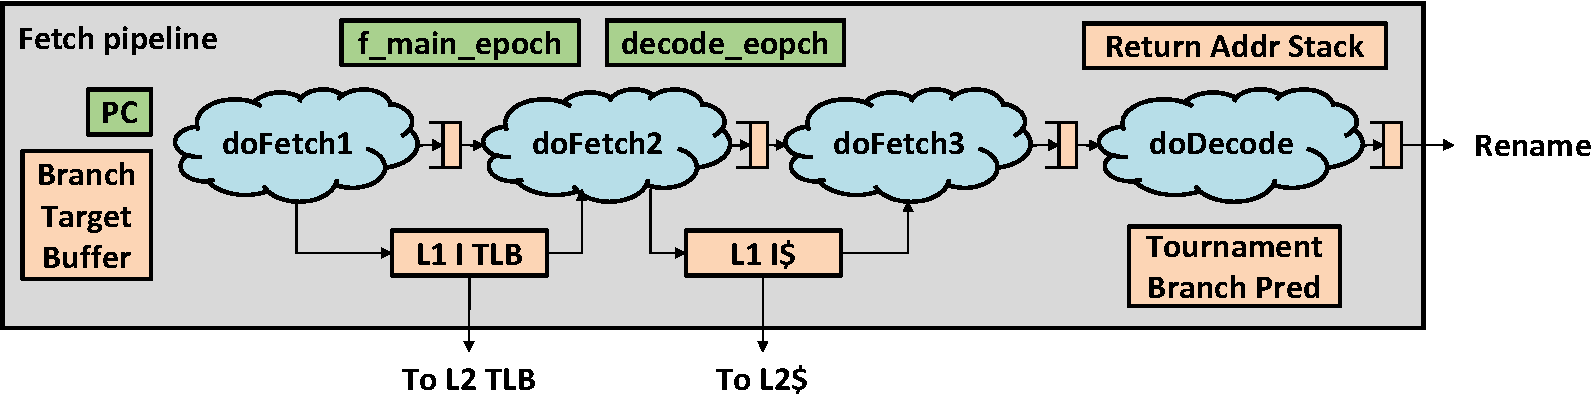
\includegraphics[width=\columnwidth]{fig/fetch_crop.pdf}
    \caption{Implementation of fetch pipeline}\label{fig:fetch-impl}
\end{figure}

Figure~\ref{fig:fetch-impl} shows the internal implementation of the fetch pipeline.
There are three internal rules:
\begin{itemize}
    \item Rule \code{doFetch1}: initiates the address translation of PC, and use BTB to update the PC.
    \item Rule \code{doFetch2}: retrieves the translated physical address and starts accessing I cache (or boot rom via the \code{mmioIfc} interface) to fetch instructions.
    \item Rule \code{doFetch3}: cuts the fetched data into a vector of instructions (because we are doing superscalar fetch).
    \item Rule \code{doDecode}: performs branch predictions and decodes instructions.
\end{itemize}
To ensure the correctness of branch redictions, the fetch pipeline contains two epochs:
\begin{itemize}
    \item EHR \code{f\_main\_epoch}: is the copy of the epoch in the epoch manager (Section~\ref{sec:epoch}), and is incremented by the \code{redirect} method.
    \item EHR \code{decode\_epoch}: is local to the fetch pipeline, and is incremented when the \code{doDecode} rule redirects PC according to branch predictors.
\end{itemize}
Rule \code{doFetch1} tag the request to I TLB with both epochs, and both epochs will flow through the pipeline with the fetched instructions.
Rule \code{doDecode} checks both epochs to drop wrong-path instructions, and only \code{f\_main\_epoch} is outputted to the rename stage with the correct-path instruction.

\subsubsection{Source Code}
See module \code{mkFetchStage} in \code{//procs/RV64G\_OOO/FetchStage.bsv}.

